\documentclass{article}

% Packages
\usepackage{amsmath} % for mathematical features
\usepackage{amsfonts} % for mathematical fonts
\usepackage{amssymb} % for mathematical symbols
\usepackage{graphicx} % for including images
\usepackage{enumerate} % for more options in lists

% Document Setup
\title{Computer Network HW1}
\author{Hsiang-Sheng Huang (CS 111062117)}
\date{\today}

% Adjust margins
\addtolength{\textwidth}{1in}
\addtolength{\topmargin}{-.5in}
\addtolength{\textheight}{1.0in}

\begin{document}
\maketitle

\section{Problem 1}
A: $4950$ links.\\

Since the diameter of a network with $100$ nodes is $1$, this is a fully connected network. That is, there are $C^{100}_2=\frac{100\times99}{2}=4950$ links.

\section{Problem 2}
A: $99$ links.\\

The optimal solution is that we place $99$ nodes as a circle and $1$ node in the center. We give $99$ links from the nodes on the circle to the center node, it makes that the diameter of the network with 100 nodes is $2$.\\

\section{Problem 3}
A: $50$.\\

The optimal solution is that we place the $100$ nodes as a circle and each node links the right node and left node, which makes that the degree of each node is $2$. Then, we know the fact that the diameter of the network is $50$.

\newpage

\section{Problem 4}
A: Impossible.\\

By the following picture, we use a greedy method to approach the goal. If the diameter of the network is $5$ and the degree of every nodes is $3$, there would be $1+3+6+12+24+48=94$ nodes on the network, which is less than $100$. So it is impossible.

\begin{figure}[htbp]
  \centering
  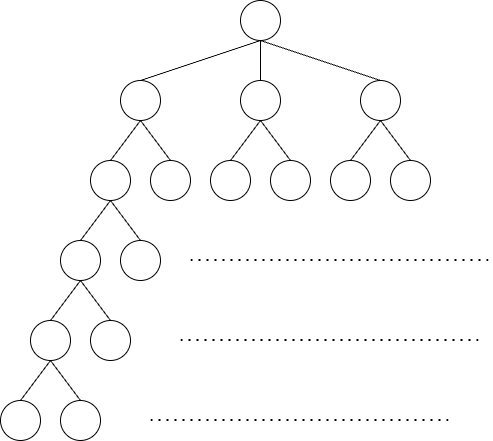
\includegraphics[width=0.5\textwidth]{001.png}
  % \caption{example}
  % \label{fig:example}
\end{figure}

\end{document}
